\documentclass{article}

\usepackage{graphicx}
\usepackage{tikz}
\usepackage{tikzsymbols}
\usetikzlibrary{calc,patterns,shapes.geometric}
\pagestyle{empty}
\usepackage[margin=0pt]{geometry}
\geometry{papersize={14in,12in}}

\def\centerarc[#1](#2)(#3:#4:#5){\draw[#1] ($(#2)+({#5*cos(#3)},{#5*sin(#3)})$) arc (#3:#4:#5);}

\begin{document}
	\begin{figure}
		\centering
		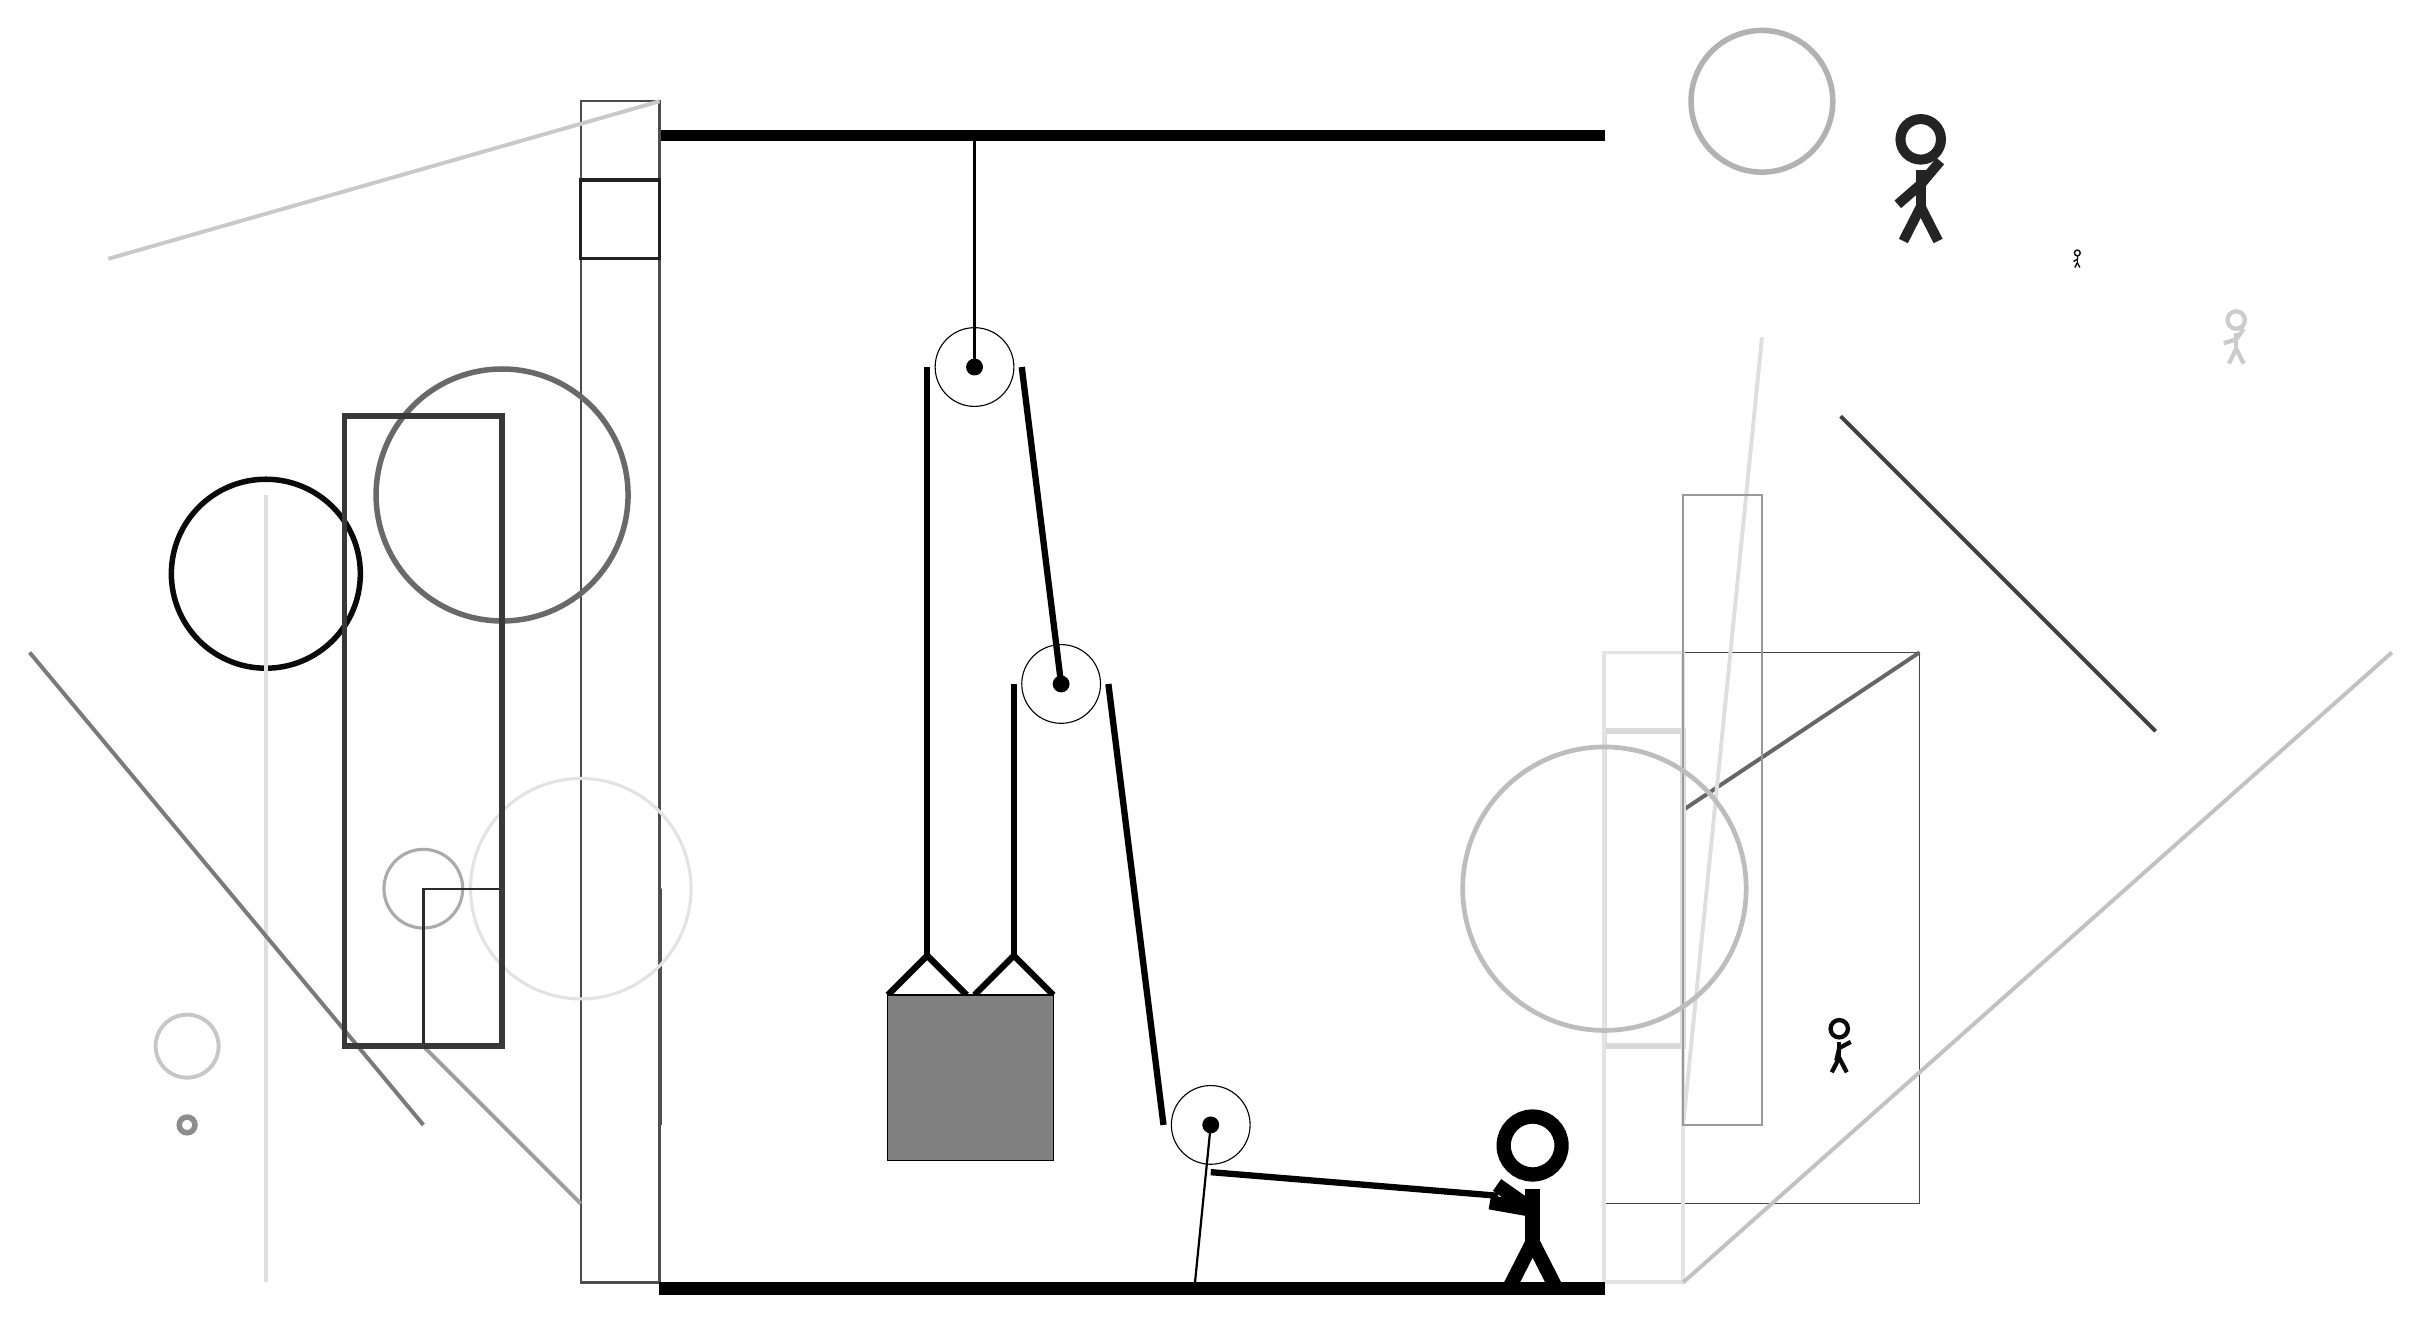
\begin{tikzpicture}
			%%%%% START %%%%%
			
			\draw[fill=black] (-2, 11.5) rectangle (10, 11.625);
			
			\draw (2, 8.625) circle (0.5);
			\draw[fill=black] (2, 8.625) circle (0.1);
			\draw[thick] (2, 8.625) -- (2, 11.5);
			
			\draw [line width=0.5mm, color=black!22](-8, 0) circle (0.4);
			
			\node[line width=0.4mm, color=black!94] at (16, 10) {\Strichmaxerl[1][28][85]};
			\draw[line width=0.5mm, color=black!75](13, 8) -- (17, 4);
			\draw[line width=0.3mm, color=black!70] (-2, 12) rectangle (-3, -3);
			\draw[line width=0.2mm, color=black!73] (10, 5) rectangle (14, -2);
			
			\draw[line width=0.5mm, color=black!60](14, 5) -- (11, 3);
			\draw[line width=0.5mm, color=black!38](-5, 0) -- (-3, -2);
			\draw [line width=0.7mm, color=black!30](12, 12) circle (0.9);
			\draw [line width=0.7mm, color=black!96](-7, 6) circle (1.2);
			\draw[line width=0.5mm, color=black!13](-7, 7) -- (-7, -3);
			
			\node[line width=0.6mm, color=black!86] at (14, 11) {\Strichmaxerl[7][41][50]};
			
			\draw[line width=0.7mm, color=black!15] (10, 4) rectangle (11, 0);
			\draw[line width=0.5mm, color=black!52](-5, -1) -- (-10, 5);
			\draw[line width=0.5mm, color=black!69] (-2, 2) rectangle (-2, -1);
			\draw [line width=0.4mm, color=black!11](-3, 2) circle (1.4);
			\draw[line width=0.5mm, color=black!13](11, -1) -- (12, 9);
			\draw[line width=0.5mm, color=black!11] (11, -3) rectangle (10, 5);
			
			\draw [line width=0.7mm, color=black!45](-8, -1) circle (0.1);
			\draw [line width=0.4mm, color=black!33](-5, 2) circle (0.5);
			\draw[line width=0.5mm, color=black!24](11, -3) -- (20, 5);
			\draw[line width=0.4mm, color=black!87] (-3, 11) rectangle (-2, 10);
			\node[line width=0.7mm, color=black!20] at (18, 9) {\Strichmaxerl[3][17][55]};
			\draw[line width=0.3mm, color=black!83] (-4, 2) rectangle (-5, 0);
			\draw[line width=0.3mm, color=black!100] (-2, 5) rectangle (-2, 5);
			\node[line width=0.4mm, color=black!96] at (13, 0) {\Strichmaxerl[3][77][28]};
			
			\draw[line width=0.5mm, color=black!21](-2, 12) -- (-9, 10);
			\draw [line width=0.7mm, color=black!59](-4, 7) circle (1.6);
			\draw[line width=0.3mm, color=black!40] (11, 7) rectangle (12, -1);
			\draw [line width=0.6mm, color=black!26](10, 2) circle (1.8);
			\draw[line width=0.7mm, color=black!78] (-4, 0) rectangle (-6, 8);
			
			\draw (3.1, 4.6) circle (0.5);
			\draw[fill=black] (3.1, 4.6) circle (0.1);
			
			\draw (5, -1) circle (0.5);
			\draw[fill=black] (5, -1) circle (0.1);
			\draw[thick] (5, -1) -- (4.8, -3);
			
			\draw[line width = 0.8mm]  (0.9, 0.65) -- (1.4, 1.15) -- (1.9, 0.65);
			\draw[line width = 0.8mm]  (2.0, 0.65) -- (2.5, 1.15) -- (3.0, 0.65);
			\draw[fill=black!50] (0.9, 0.65) rectangle (3.0, -1.45);
			
			\draw[line width = 0.8mm] (1.4, 8.625) -- (1.4, 1.15);
			\centerarc[line width = 0.8mm](2, 8.625)(0:180:0.6);
			\draw[line width = 0.8mm] (2.6, 8.625) -- (3.1, 4.6);
			\draw[line width = 0.8mm] (2.5, 4.6) -- (2.5, 1.15);
			\centerarc[line width = 0.8mm](3.1, 4.6)(0:180:0.6);
			\draw[line width = 0.8mm] (3.7, 4.6) -- (4.4, -1);
			\centerarc[line width = 0.8mm](5, -1)(180:270:0.6);
			\draw[line width = 0.8mm] (5, -1.6) -- (8.65, -1.9);
			
			\node at (9, -2) {\Strichmaxerl[10][-35][170]};
			
			\draw[fill=black] (-2, -3) rectangle (10, -3.15);
			
			%%%%% END %%%%%
		\end{tikzpicture}
	\end{figure}	
\end{document}